\documentclass[11pt,letterpaper]{article}
\usepackage[margin=1in]{geometry}
\usepackage[T1]{fontenc}
\usepackage[utf8]{inputenc}
\usepackage{lmodern}
\usepackage{longtable,booktabs,array,enumitem,hyperref,xcolor,graphicx,pdflscape}
\usepackage{indentfirst}
\usepackage{fancyhdr}
\usepackage{graphicx}
\usepackage{titling}
\usepackage{enumitem}
\hypersetup{colorlinks=true,linkcolor=blue,urlcolor=blue}
\setlist[itemize]{leftmargin=*}

% Automatically prefixes the section number to all first-level enumerate lists
% label=\thesubsection.\arabic* pulls "1.1" and adds the list item number
% leftmargin=3\parindent indents 3 paragraphs.
\setlist[enumerate,1]{label=\thesubsection.\arabic*,leftmargin=\parindent}

\pagestyle{fancy}
\geometry{a4paper, margin=1in}

\newcommand{\myTitle}{Golden Eagle Flight Plan Workflow Diagram}

\begin{document}

\title{Golden Eagle Flight Plan\\Workflow Diagram\\CS 3338 Final Project}
\author{Project Group 26\\Jason Reese \\ Juan Torres Llamas \\ Victor Hernandez}
\date{November 19, 2026}

\newpage %
\maketitle

\newpage %

\begin{table}[h!]
\centering
\caption{\textbf{Revision History}}
\begin{tabular}{|c|c|c|c|}
\hline
\textbf{Name} & \textbf{Date} & \textbf{Reasons for Changes} & \textbf{Version} \\
\hline
Project Group 26 & 11/17/2026 & First Draft & 1.0.0 \\
\hline
Project Group 26 & 11/19/2026 & Snapshot 1 update & 1.1.0 \\
\hline
\end{tabular}
\end{table}

\newpage %

\begin{center}Design draft --- November 2026\end{center}
\tableofcontents
\newpage %

\fancyhf{}
\pagestyle{fancy}
\fancyhead[L]{\myTitle}
\fancyhead[R]{Page \thepage}
\fancyfoot[C]{}

\newpage %



\section{Introduction}
This document shows the planned Snapshot 1 account workflow and the data flow in the current development starter. It follows the user roles and access rules described in the team's SRS and SDD.

\section{Snapshot 1 Workflow}
\begin{center}
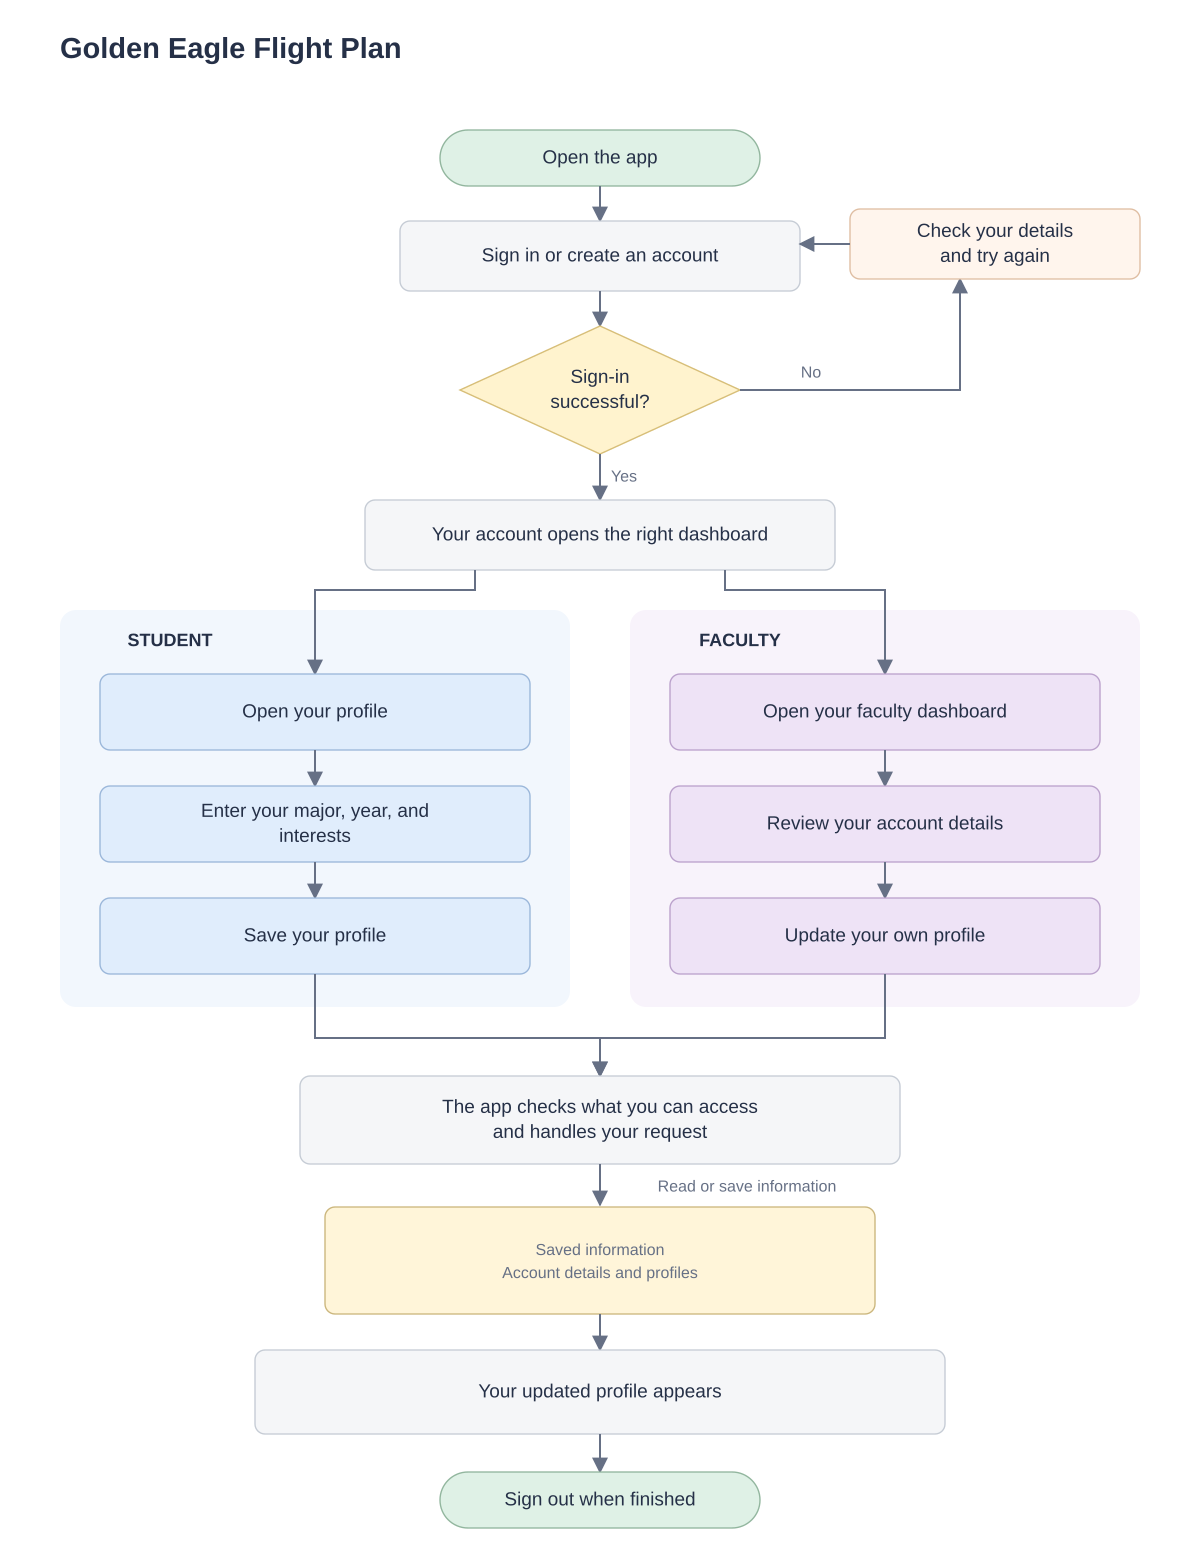
\includegraphics[width=0.82\textwidth,height=0.76\textheight,keepaspectratio]{workflow.png}
\end{center}

\newpage
\section{How the Workflow Works}
A student or faculty member opens the application and signs in or creates an account. If sign-in fails, the user checks their details and tries again. A successful sign-in opens the homepage for that account. The diagram uses the student and faculty paths to show the main profile workflow.

\subsection{Account Types}
The full account design includes students, faculty, student organizations, and administrators. Faculty and student organization registrations require administrator approval. Administrators also control the assignment of restricted roles. Those approval steps are defined in the SRS and SDD; the diagram summarizes the main account journey.

\subsection{Saved Information and Access}
The server checks account permissions before reading or saving protected information. Students can access their own profiles, while faculty and administrators can access student profiles according to the requirements. Student organizations cannot view student profiles. Database access is handled by the server rather than directly by the browser.

The planned database separates users, roles, and profiles. After an allowed operation, the application displays the result. Users sign out when finished.

\section{Current Starter Data Flow}
The current source code does not implement account registration or login yet. It provides the development foundation:
\begin{enumerate}[label=\arabic*.]
\item A user opens the React frontend at \url{http://localhost:3000}.
\item The browser sends a request to the Express backend at \url{http://localhost:5001}.
\item The backend inserts a visit into PostgreSQL and reads the total visit count.
\item The backend returns the greeting and count to the frontend.
\item The frontend displays the result. If the request fails, it displays that the backend could not be reached.
\end{enumerate}
Docker Compose connects the frontend, backend, and database services. The database stores visit records in the \texttt{db-data} volume. This starter page is available without a login and does not contain student account or profile records.

\section{Revisions at Later Snapshots}
The diagram and this explanation will be updated when account features are implemented and when later snapshots introduce additional user actions or data flows. The Mermaid source is stored in \texttt{workflow.mmd}; PNG and SVG versions are included for the manual and GitHub README.

\end{document}
